%\lipsum[4-4]
This chapter presents the context, motivation and document structure of a study of outlier detection in a railways WSN-based smart grid. 

\section{Context and motivation of PhD}

The railway system is responsible for 1.3\% of entire European energy consumption, \cite{iea-uic2016}. 
The discussion of the energy efficiency in railways is a grown topic due to its contribution to the global energy consumption.

The energy efficiency analysis and management requires a detailed mapping of the energy consumption/generation in the railway system. 

This detailed mapping of the energy flows should include, not only the rolling stock level but also the traction substations and the auxiliary services.

The knowledge of all the load curves permits the load prevision, peak shaving and energy cost optimization for all global railway system.


\section{Shift2Rail Framework}

This work is supported by the iRail PhD programme – Innovation in Railway Systems and Technologies whose objectives are aligned with the Shift2Rail objectives, \cite{shift2rail2015}: 

\begin{itemize}
		\setlength\itemsep{-0.5em}
		\item 1. Cutting the life-cycle cost of railway transport by as much as 50\%;
		\item 2. Doubling the railway capacity;
		\item 3. Increasing the reliability and punctuality by as much as 50\%.
\end{itemize}


Framed on the Shift2Rail (S2R) Innovation Programme 3 (IP3) with the focus on ”Cost efficient and reliable infrastructure”, it is proposed to develop a Smart Metering Demonstrator (SMD) that reach a detailed monitoring and supervision of various energy flows on the premises of embrace the entire Railway System.

\begin{figure}[h!]
	\centering
	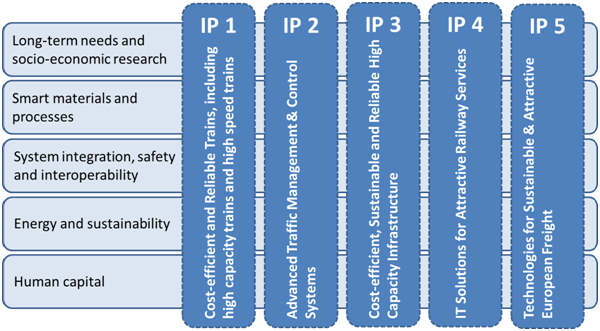
\includegraphics[width=0.60\textwidth,keepaspectratio]{figures/IPs}
	\caption{Shif2Rail Inovation Programmes. }
	\label{fig:ips}
\end{figure}

The purpose of any energy management strategy is to build the dynamics of every loads and generators of the power system. 

This should be performed based on an extensive knowledge of every energy flows. 

This way, the SMD is required to propose and validate a standard metering architecture that involves the coordination of every measurements either in on-board and in ground. 
In advance, energy data analysis should be provided based on relevant stored data. 

\section{PhD state of the art}

This section will cover a summary of the state of the art that supports this PhD.

Based on the state of the art, current metering systems focus on rolling stock on-board energy meters for energy billing purposes only, where the metering devices are located close to the pantograph, \cite{shift2rail2015}.

An advance beyond the state of the art is the expansion of the measurement system at railway system level, making it a distributed one, including both on-board and track-side measurements, thus achieving detailed mappings. 

\vspace{2em}

Other point in the state of the art is the intrusion level of currently used metering systems, that in one way, became a critical subsystem of the rolling stock and in other way, requires relatively long implementation, \cite{shift2rail2015}. 

An advance beyond the state of the art is a solution based on non-intrusive technology. More detailed simulation models in conjunction with field measurements is the methodology to be investigated.



%\textbf{\textit{Research Plan}}

Specific challenges and requirements of this research are the development of non-intrusive Wireless Sensor Networks (WSN)  in the railway environment. 
It is intended that this technology should be based on an open system and open interfaces for the data collection, aggregation and analysis. 
Issues like metering redundancy, outlier detection, fault tolerance and communication reliability, should be considered during the research.
In addition, it is expected to design and specify a set of user applications.
Those applications are focused in the energy analysis process with the aim of providing more information and detailed knowledge.
It is expected that this detailed knowledge would be useful in a decision support system related with, in e.g., eco-driving strategies, timetable planning and preventive maintenance.

\section{Influence of outliers in a railway remote monitoring system}
	%Outlier Detection towards improving fault tolerance and communication reliability of SMD}

Having in mind the state of the art that was previously presented in section 1.3, an important contribution of a wireless sensor network in the railway system is the availability of useful knowledge of the energy consumption to the decision support systems.

Therefore, such acquisition systems are required to provide accurate data regardless of the quality of the acquisition sensors, electromagnetic influences (EMI), sensor supply fluctuations, among others.

Through computational algorithms, the increasing of communication reliability and fault tolerance is possible. Those computational algorithms detect outliers or, in the scope of this PhD, detect erroneous data that will perturb the outcomes of decision support systems. Further on in chapter 2, this thematic is extensively explored.

\section{Document structure}

This document is divided in 5 chapters, each of them incorporate the relevant subsections to present the subjects mentioned. 
%contains several subsections according to the subjects mentioned.

\begin{table}[!h]
    \label{tb:struct}
    \centering
    \caption{Document structure}
    \vspace{0.2em}
    \begin{tabular}{c|l}%{C{2cm}|C{9cm}}
    \textbf{Chapter} & \textbf{Title}                    \\ \hline
    1       &                   Introduction             \\ \hline
  %  2       &                   Railways Remote Monitoring Systems       \\ \hline
    2       &                   Outliers Detection    \\ \hline
    3       &                   Future Research    \\ \hline
    4       &                   Conclusions               \\
    \end{tabular}
\end{table}